\section{Identity}
\hypertarget{sec:Distribution:Anaconda:Firstboot:Identity}{}
\label{sec:Distribution:Anaconda:Firstboot:Identity}

\begin{description}
\item[framework:]
trunk/Identity/Themes/\$THEME/Distro/Anaconda/Firstboot/
\end{description}

\noindent Here is where CentOS firstboot design templates and image
rendering take place. Firstboot identity file structure is illustrated
in \autoref{fig:Distribution:Anaconda:Firstboot:Identity} and
described in the following sections.

\begin{figure}
\hrulefill
\begin{verbatim}
trunk/Identity/Themes/$THEME/Distro/Anaconda/Firstboot/
|-- img
|   |-- 3
|   |   `-- splash-small.png
|   |-- 4
|   |   `-- splash-small.png
|   |-- 5
|   |   `-- splash-small.png
|   |-- ... (more releases here)
|   `-- firstboot-left.png
|-- render.sh
`-- tpl
    |-- firstboot-left.svg
        `-- splash-small.svg
\end{verbatim}
\hrulefill
\caption{Firstboot identity framework.%
   \label{fig:Distribution:Anaconda:Firstboot:Identity}}
\end{figure}

\subsection{Design Templates}

\begin{description}
\item[framework:]
trunk/Identity/Themes/\$THEME/Distro/Anaconda/Firstboot/Tpl/
\end{description}

\noindent Here is where Firstboot design templates are stored.
Firstboot design templates control Firstboot's visual style. 

\begin{description}

\item[firstboot-left.svg:] This design is common for all major
releases of CentOS Distribution. It is visible in all firstboot
screens. In
\autoref{fig:Distribution:Anaconda:Firstboot:Identity:Models}, this
design is illustraded by the number 8.

\item[splash-small.svg:] This design is specific for each major
release of CentOS Distribution.  There is one splash-small.png image
for each major release of CentOS Distribution. This image is visible
only in the first (Welcome) screen of Firstboot. In
\autoref{fig:Distribution:Anaconda:Firstboot:Identity:Models}, this
design is illustraded by number 5.

\end{description}

\subsection{Design Models}

\begin{description}
\item[framework:]
trunk/Identity/Models/Distro/Anaconda/Firstboot/
\end{description}

\noindent Here is where firstboot design models are stored. Firstboot
design model is shown in
\autoref{fig:Distribution:Anaconda:Firstboot:Identity:Models} and described
below: 

\begin{figure}
\begin{center}
\fbox{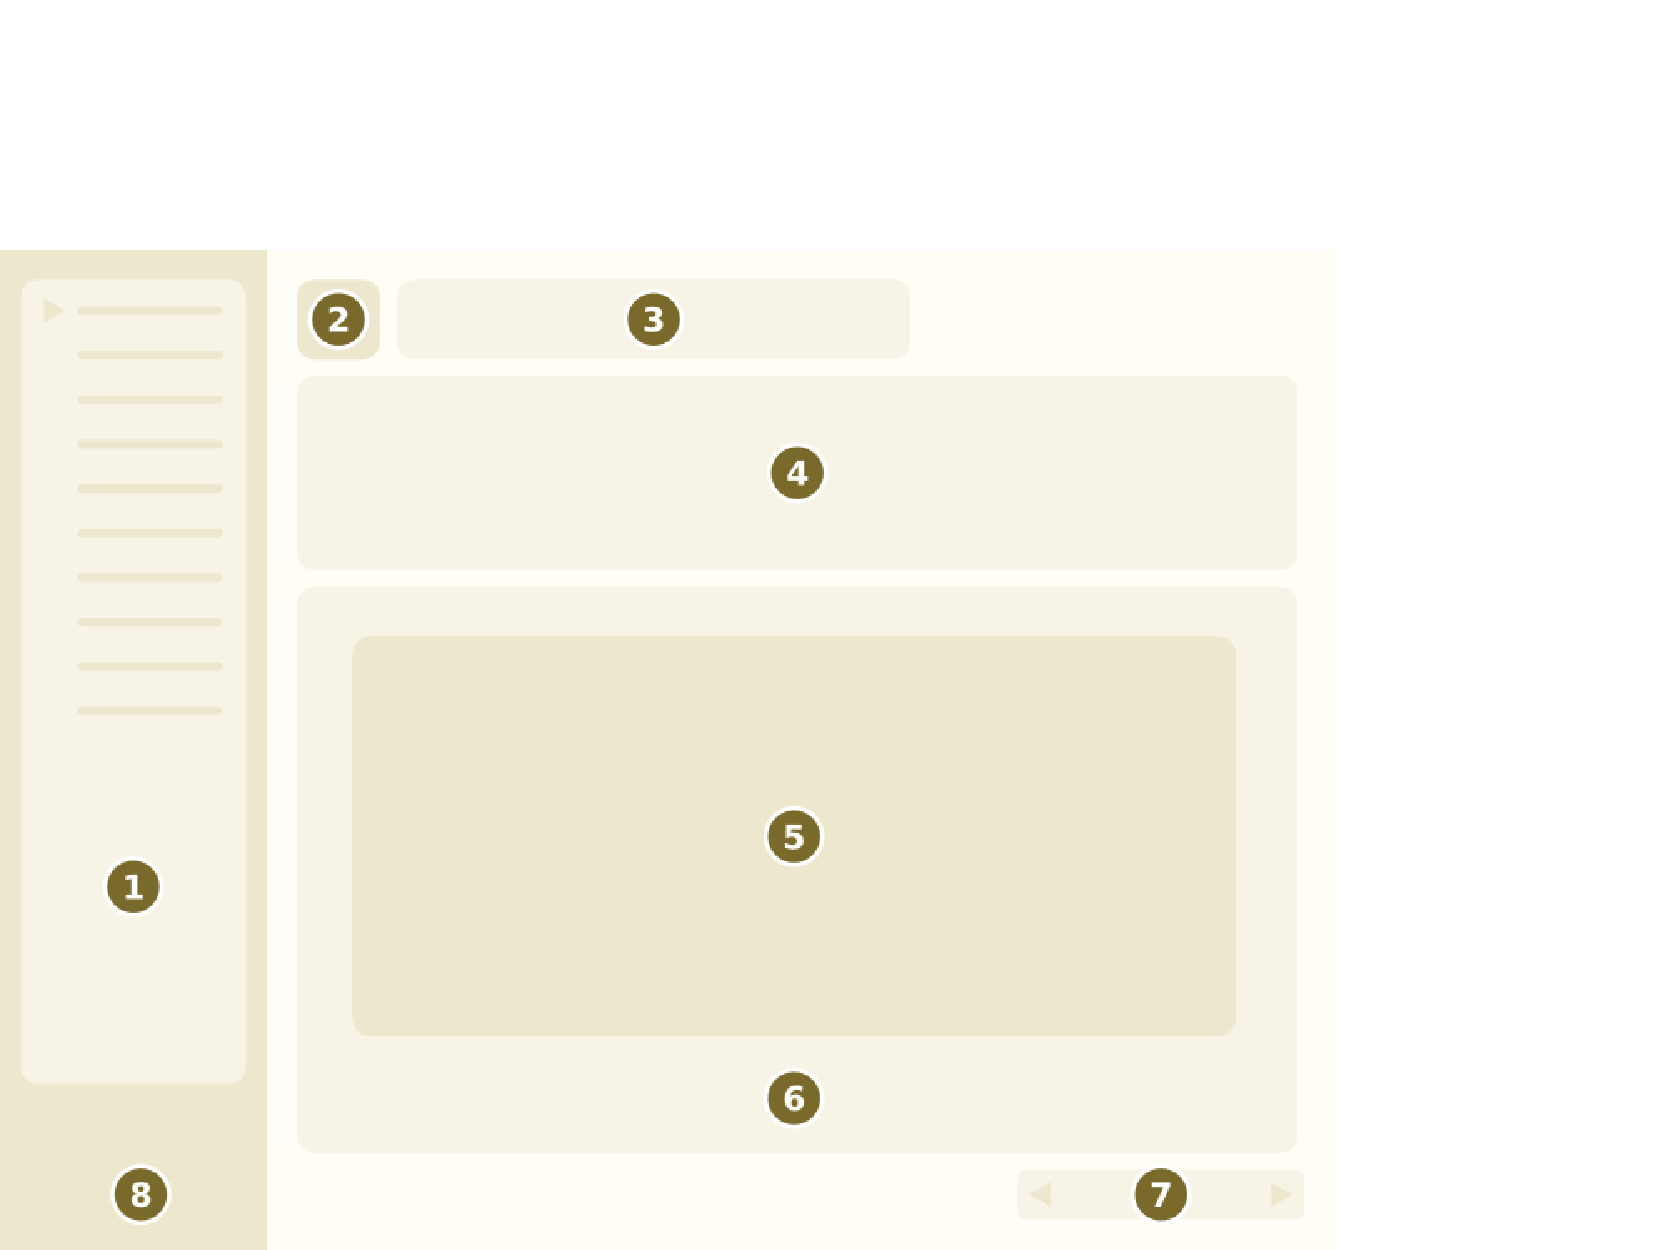
\includegraphics[width=0.8\textwidth]{%
../Identity/Models/Img/en/Distro/Anaconda/Firstboot/splash-small.pdf}}
\end{center}
\caption{Firstboot design model.%
   \label{fig:Distribution:Anaconda:Firstboot:Identity:Models}}
\end{figure}

\begin{description}

\item[1:] List of labels and a pointer showing in which configuration
screen you are.

\item[2:] Screen icon. The screen icon is visible in all firstboot
screens. Each firsboot screen may have its own screen icon.

\item[3:] Screen label.

\item[4:] Screen description. 

\item[5:] Splash image (splash-small.png). The splash
image is visible in firstboot welcome screen only.

\item[6:] Configuration stuff.

\item[7:] Navigation area. Basically two buttons to navegate
configuration back and forward.

\item[8:] List of labels' background image (firtboot-left.png).  This
image is visible in all firstboot screens.

\end{description}

\subsection{Image Files}
\hypertarget{sec:Distribution:Anaconda:Firstboot:Identity:Images}{}
\label{sec:Distribution:Anaconda:Firstboot:Identity:Images}

\begin{description}
\item[framework:]
trunk/Identity/Themes/\$THEME/Distro/Anaconda/Firstboot/Img/
\end{description}

\noindent Here is where firstboot final images are stored. 

\subsection{Image Files Rendering}
\hypertarget{sec:Distribution:Anaconda:Firstboot:Identity:ImagesRendering}{}
\label{sec:Distribution:Anaconda:Firstboot:Identity:ImagesRendering}

\begin{description}
\item[framework:]
trunk/Identity/Themes/\$THEME/Distro/Anaconda/Firstboot/
\end{description}

\noindent Here is where you produce firstboot images. The following
rendering examples, based on
\autoref{fig:Distribution:Anaconda:Firstboot:Translations}, illustrate
the firstboot image files rendering process.\\
\\
\fbox{\texttt{./render.sh}}\\
\\
\fbox{\texttt{./render.sh '(5|6)/splash'}}\\
\\
\fbox{\texttt{./render.sh '(firstboot-left|5|4)/splash'}}

\section{Translations}
\hypertarget{sec:Distribution:Anaconda:Firstboot:Translations}{}
\label{sec:Distribution:Anaconda:Firstboot:Translations}

\begin{description}
\item[framework:]
trunk/Translations/Identity/Themes/Distro/Anaconda/Firstboot
\end{description}

\noindent Here is where translators locale firstboot images. Image
localization is defined inside .sed files, also known as translation
files.  Translation files can be common or specific. The given
organization of translation files defines the translation path.

\begin{figure}[!hbp]
\hrulefill
\begin{verbatim}
trunk/Translations/Identity/Themes/Distro/Anaconda/Firstboot
|-- 3
|   `-- splash-small.sed
|-- 4
|   `-- splash-small.sed
|-- 5
|   `-- splash-small.sed
|-- ... (more release directories)
`-- firstboot-left.sed
\end{verbatim}
\hrulefill
\caption{Firstboot translation path.%
   \label{fig:Distribution:Anaconda:Firstboot:Translations}}
\end{figure}

\subsection{Translation Markers}

In firstboot, markers are used in the file splash-small.svg only,
specifically to set the major release number of CentOS Distribution in
CentOS Release Brand. Since firstboot-left.svg design is common for
all CentOS Distribution there is no need to set any marker on it.

Markers used in firstboot design templates and translation files are
described in \autoref{tab:Distribution:Anaconda:Firstboot:Markers}.

\begin{table}
\centering
\begin{tabular}{rl}
\hline
\textbf{Marker} & \textbf{Description}\\
\hline
=MAJOR\_RELEASE= & Major release number of CentOS Distribution.\\
\hline
\end{tabular}
\caption{Firstboot translation markers.%
   \label{tab:Distribution:Anaconda:Firstboot:Markers}}
\end{table}

\section{Manuals}
\hypertarget{sec:Distribution:Anaconda:Firstboot:Manuals}{}
\label{sec:Distribution:Anaconda:Firstboot:Manuals}

\begin{description}
\item[framework:]
trunk/Manuals/Distribution/Anaconda/Firstboot/
\end{description}

\noindent Here is where firstboot documentation is stored.  If you
want to help improving Firstboot documentation this is the place you
need to go.

\section{Scripts}
\hypertarget{sec:Distribution:Anaconda:Firstboot:Scripts}{}

\begin{description}
\item[framework:] trunk/Scripts/Config/Identity/Themes/Distro/Anaconda/Firstboot/
\end{description}

\noindent Here is stored the Firstboot \texttt{render.conf.sh}
configuration script.  To render Firstboot images correctly, the
\texttt{ARTCOMP} configuration variable inside Anaconda progress
configuration script should be defined as illustrated in
\autoref{fig:Distribution:Anaconda:Firstboot:Scripts:Config}. 

\begin{figure}
\hrulefill
\begin{verbatim}
# Define artwork component.
ARTCOMP='Identity/Themes/Distro/Anaconda/Firstboot'
\end{verbatim}
\hrulefill
\caption{Firstboot configuration layout.%
   \label{fig:Distribution:Anaconda:Firstboot:Scripts:Config}}
\end{figure}

